\section{Jeu de données et analyse exploratoire}

\subsection{Description du jeu de données}

Le jeu de données utilisé dans cette étude est composé de séries temporelles
multivariées collectées à partir d'un réseau urbain de distribution d'eau sur
une période de surveillance d'environ trois semaines (janvier 2024). Les
données incluent des mesures provenant de dix capteurs, couvrant des variables
hydrauliques clés telles que la pression et le débit, ainsi que des variables
environnementales, notamment la température.

Après prétraitement et suppression des événements de rupture anormaux, le jeu
de données contient un total de 5{,}590 échantillons, dont 774 correspondent à
des événements de fuite, soit environ 13.8\% des données. Ce déséquilibre de
classes reflète les conditions réelles, où les occurrences de fuite sont
relativement rares par rapport au fonctionnement normal du système.

Chaque observation est associée à une étiquette binaire indiquant la présence
ou l'absence d'une fuite. Pour permettre un apprentissage supervisé, les
données sont ensuite transformées en séquences de longueur fixe au moyen d'une
approche par fenêtre glissante.

\subsection{Analyse des distributions}

Afin de mieux comprendre les caractéristiques des données, nous analysons d'abord
la distribution des variables clés en conditions normales et en conditions de fuite.

\begin{figure}[h]
\centering
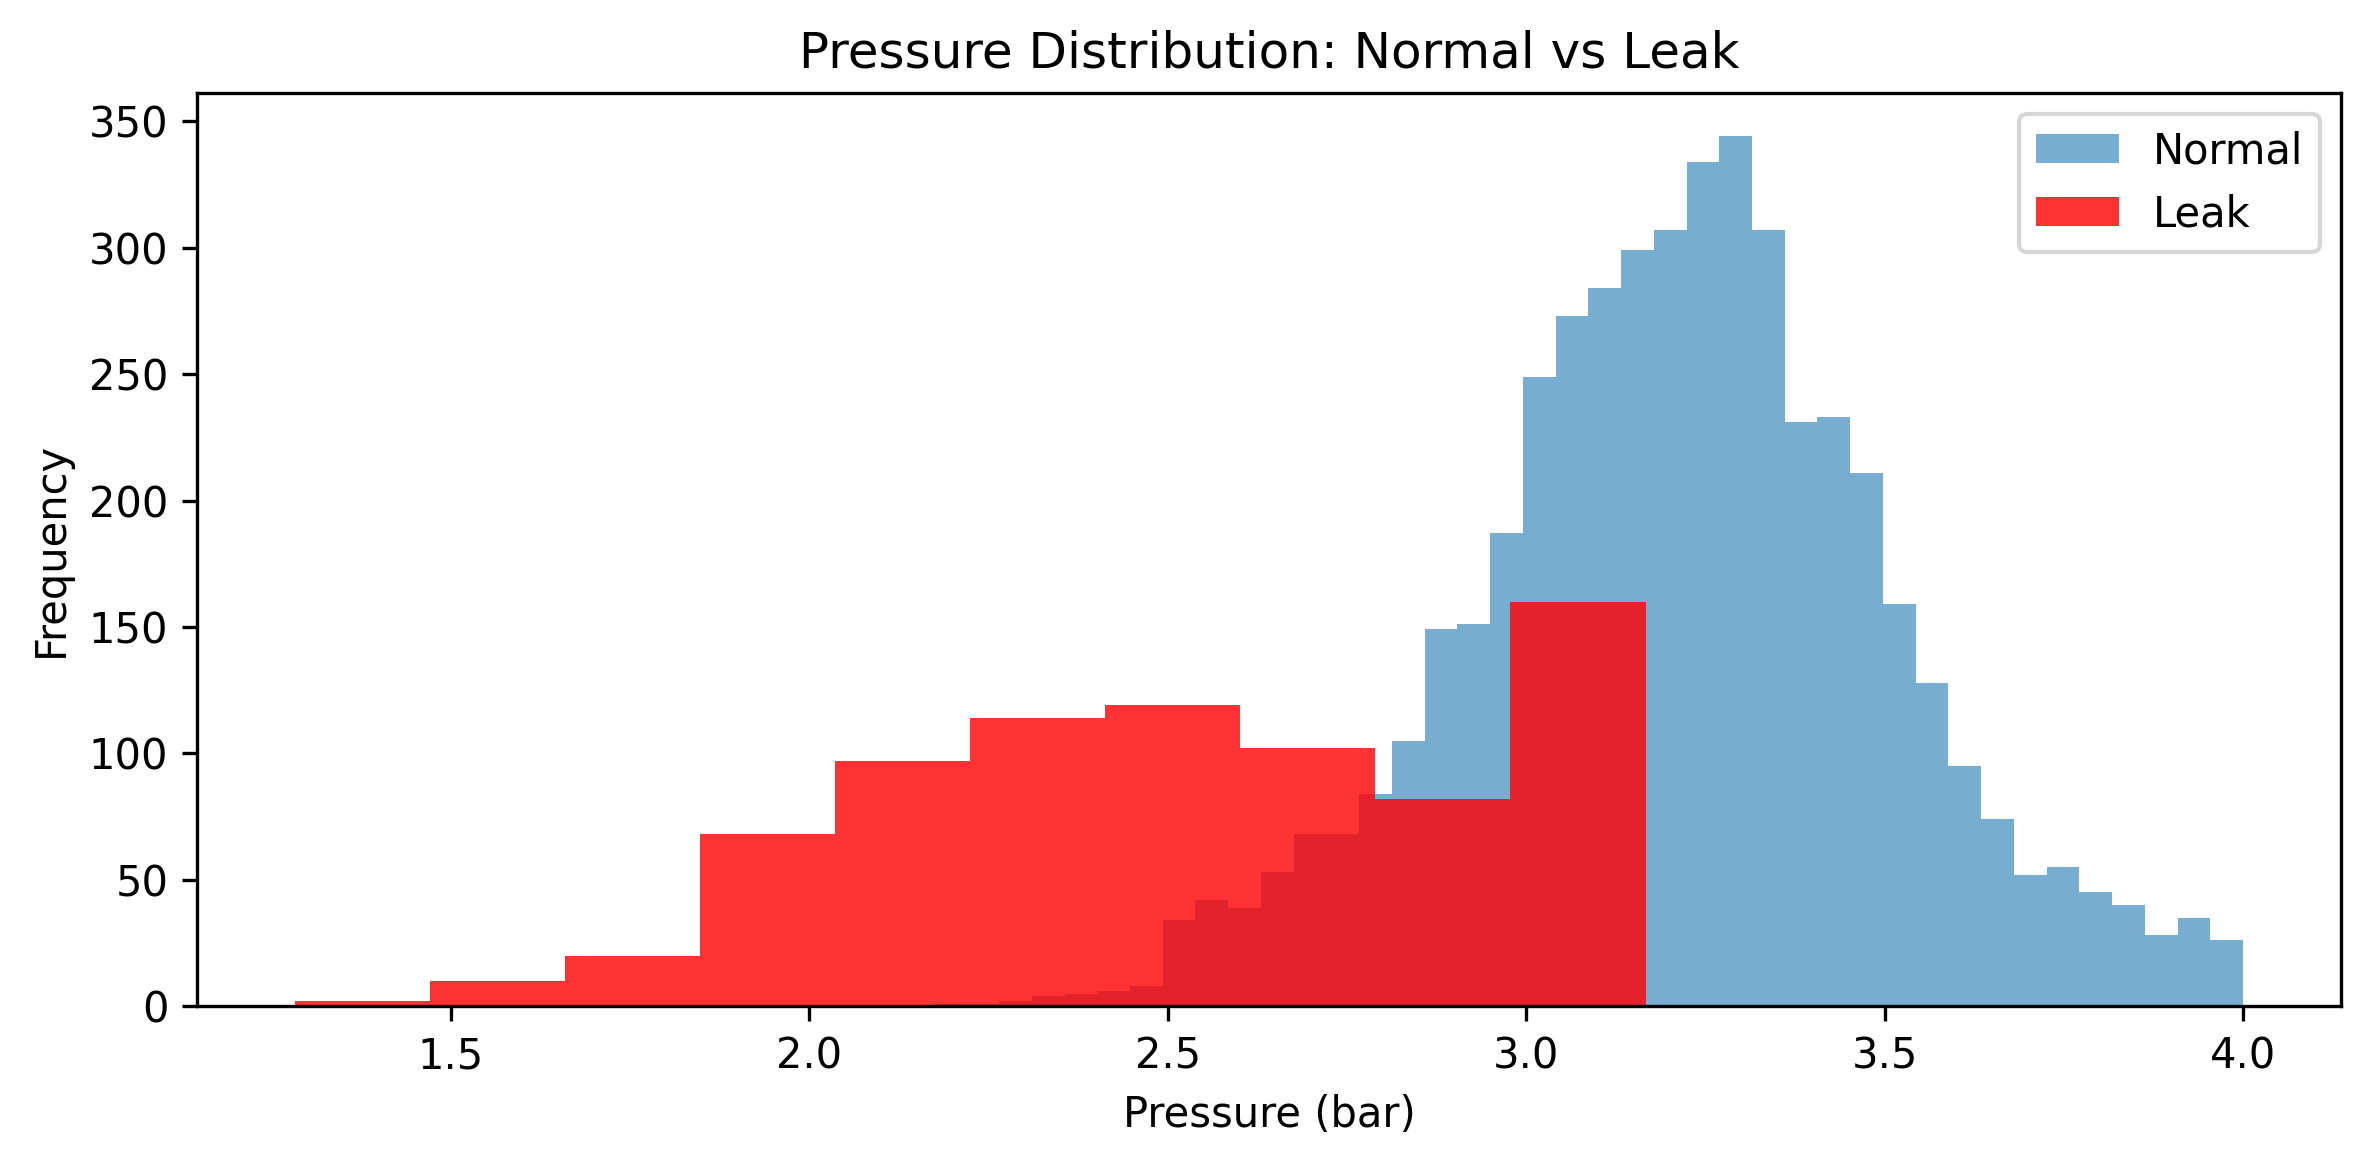
\includegraphics[width=0.9\columnwidth]{images/fig1_pressure_distribution.png}
\caption{Distribution de la pression en conditions normales et de fuite.}
\label{fig:pressure_distribution}
\end{figure}

Comme le montre la Figure~\ref{fig:pressure_distribution}, les valeurs de
pression pendant les événements de fuite sont systématiquement plus faibles que
celles observées en fonctionnement normal. Ce décalage reflète le comportement
hydraulique sous-jacent, où les fuites induisent des chutes de pression dans le
réseau.

\begin{figure}[h]
\centering
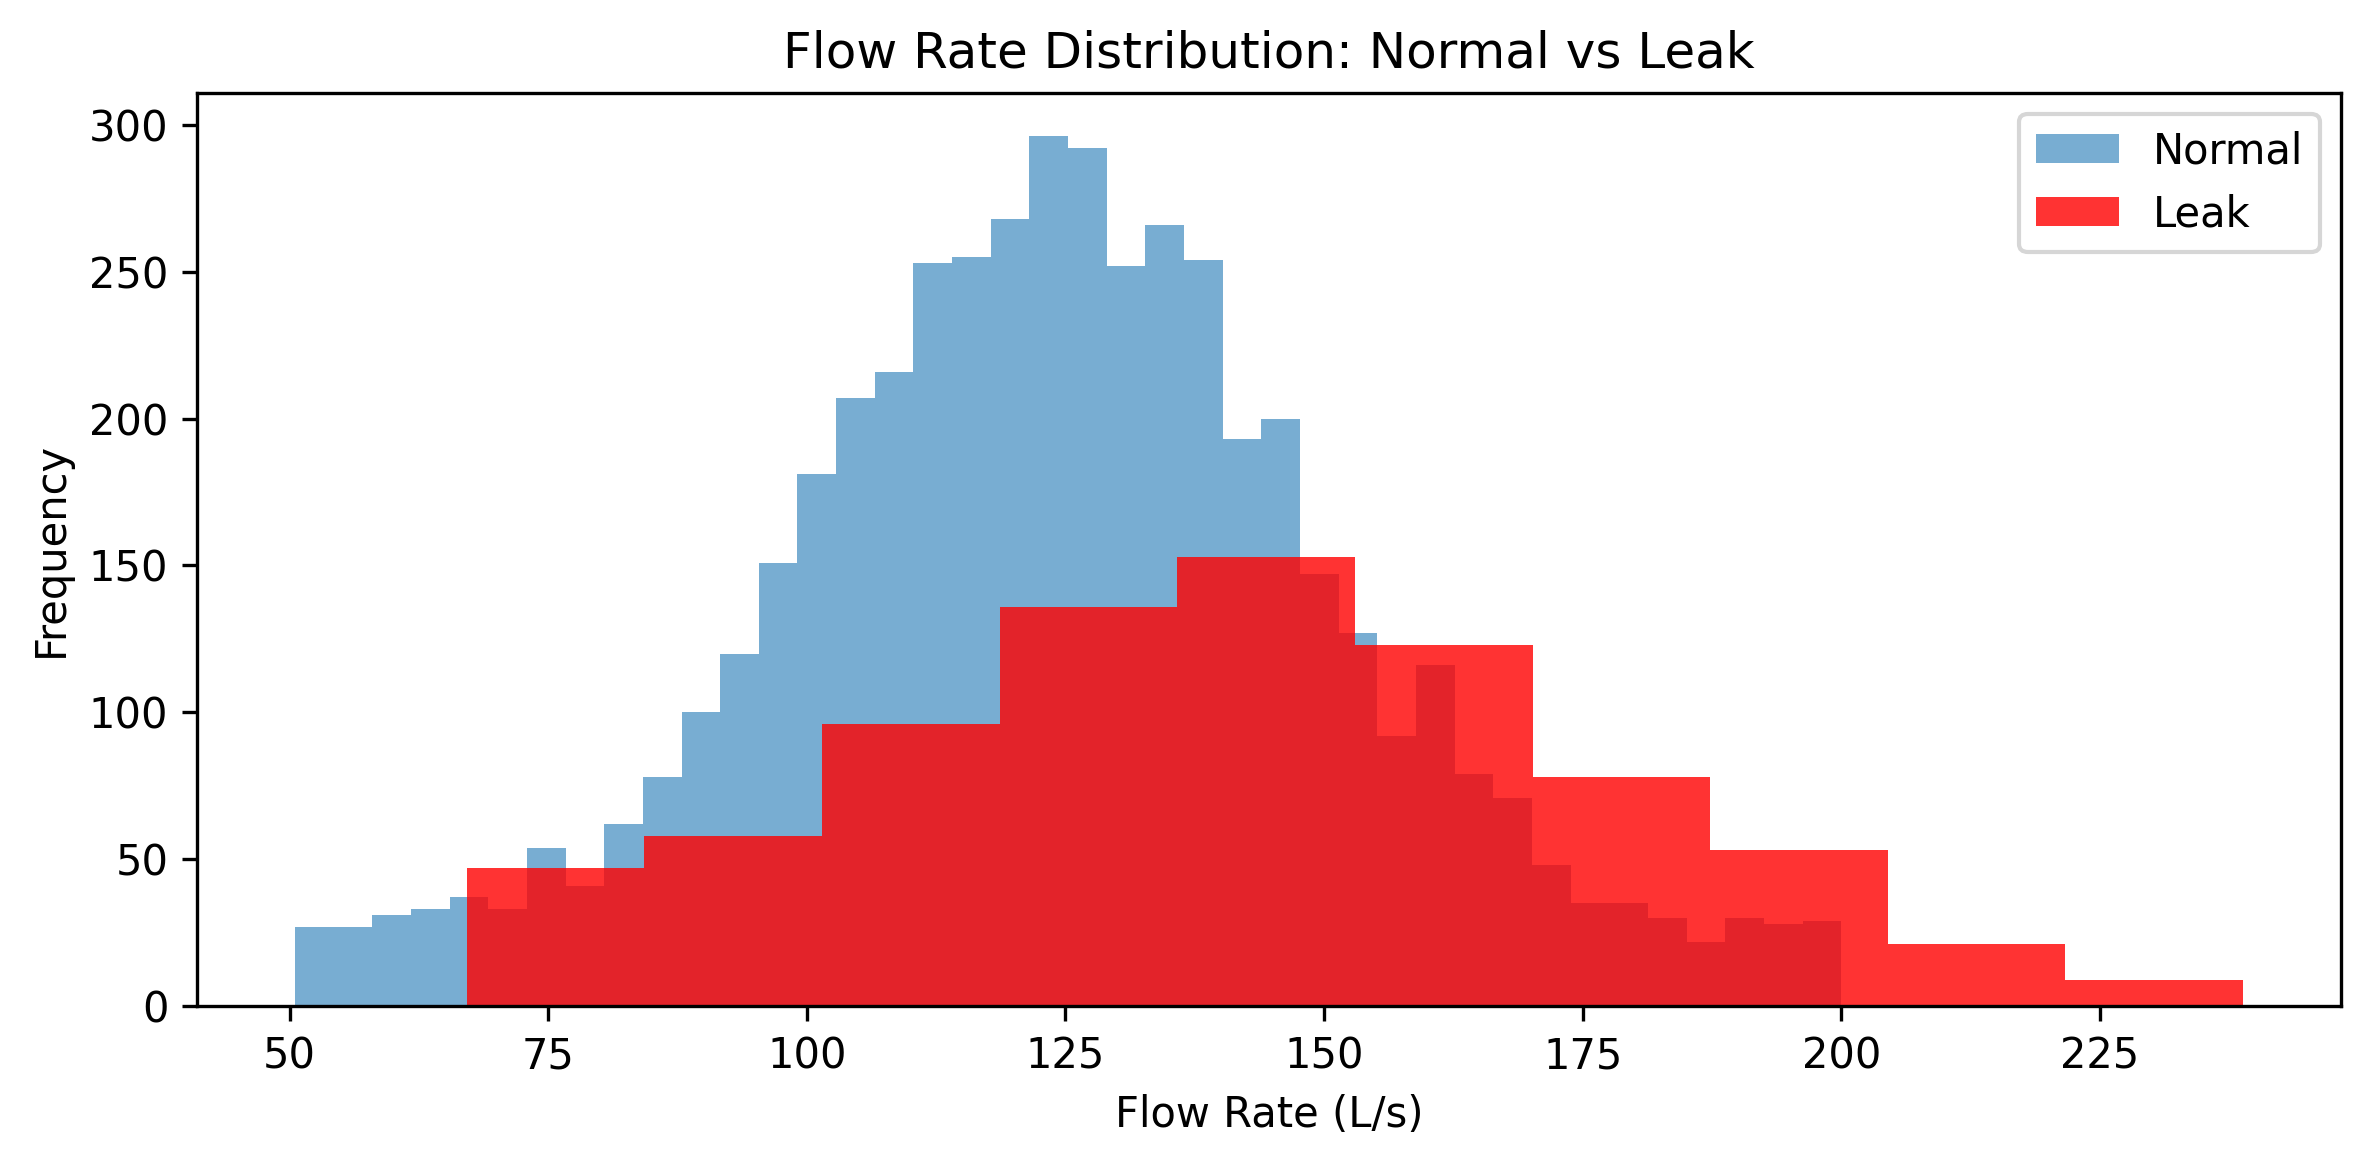
\includegraphics[width=0.9\columnwidth]{images/fig2_flowrate_distribution.png}
\caption{Distribution du débit en conditions normales et de fuite.}
\label{fig:flow_distribution}
\end{figure}

La Figure~\ref{fig:flow_distribution} montre que les valeurs de débit présentent
une variabilité plus importante et une légère augmentation en conditions de fuite.
Ce comportement est cohérent avec l'augmentation attendue de l'écoulement d'eau
associée aux fuites, conduisant à des profils de débit plus dispersés.

\subsection{Comportement temporel des événements de fuite}

Pour analyser les dynamiques temporelles, nous examinons des séries temporelles
au niveau capteur avec annotation des événements de fuite.

\begin{figure}[h]
\centering
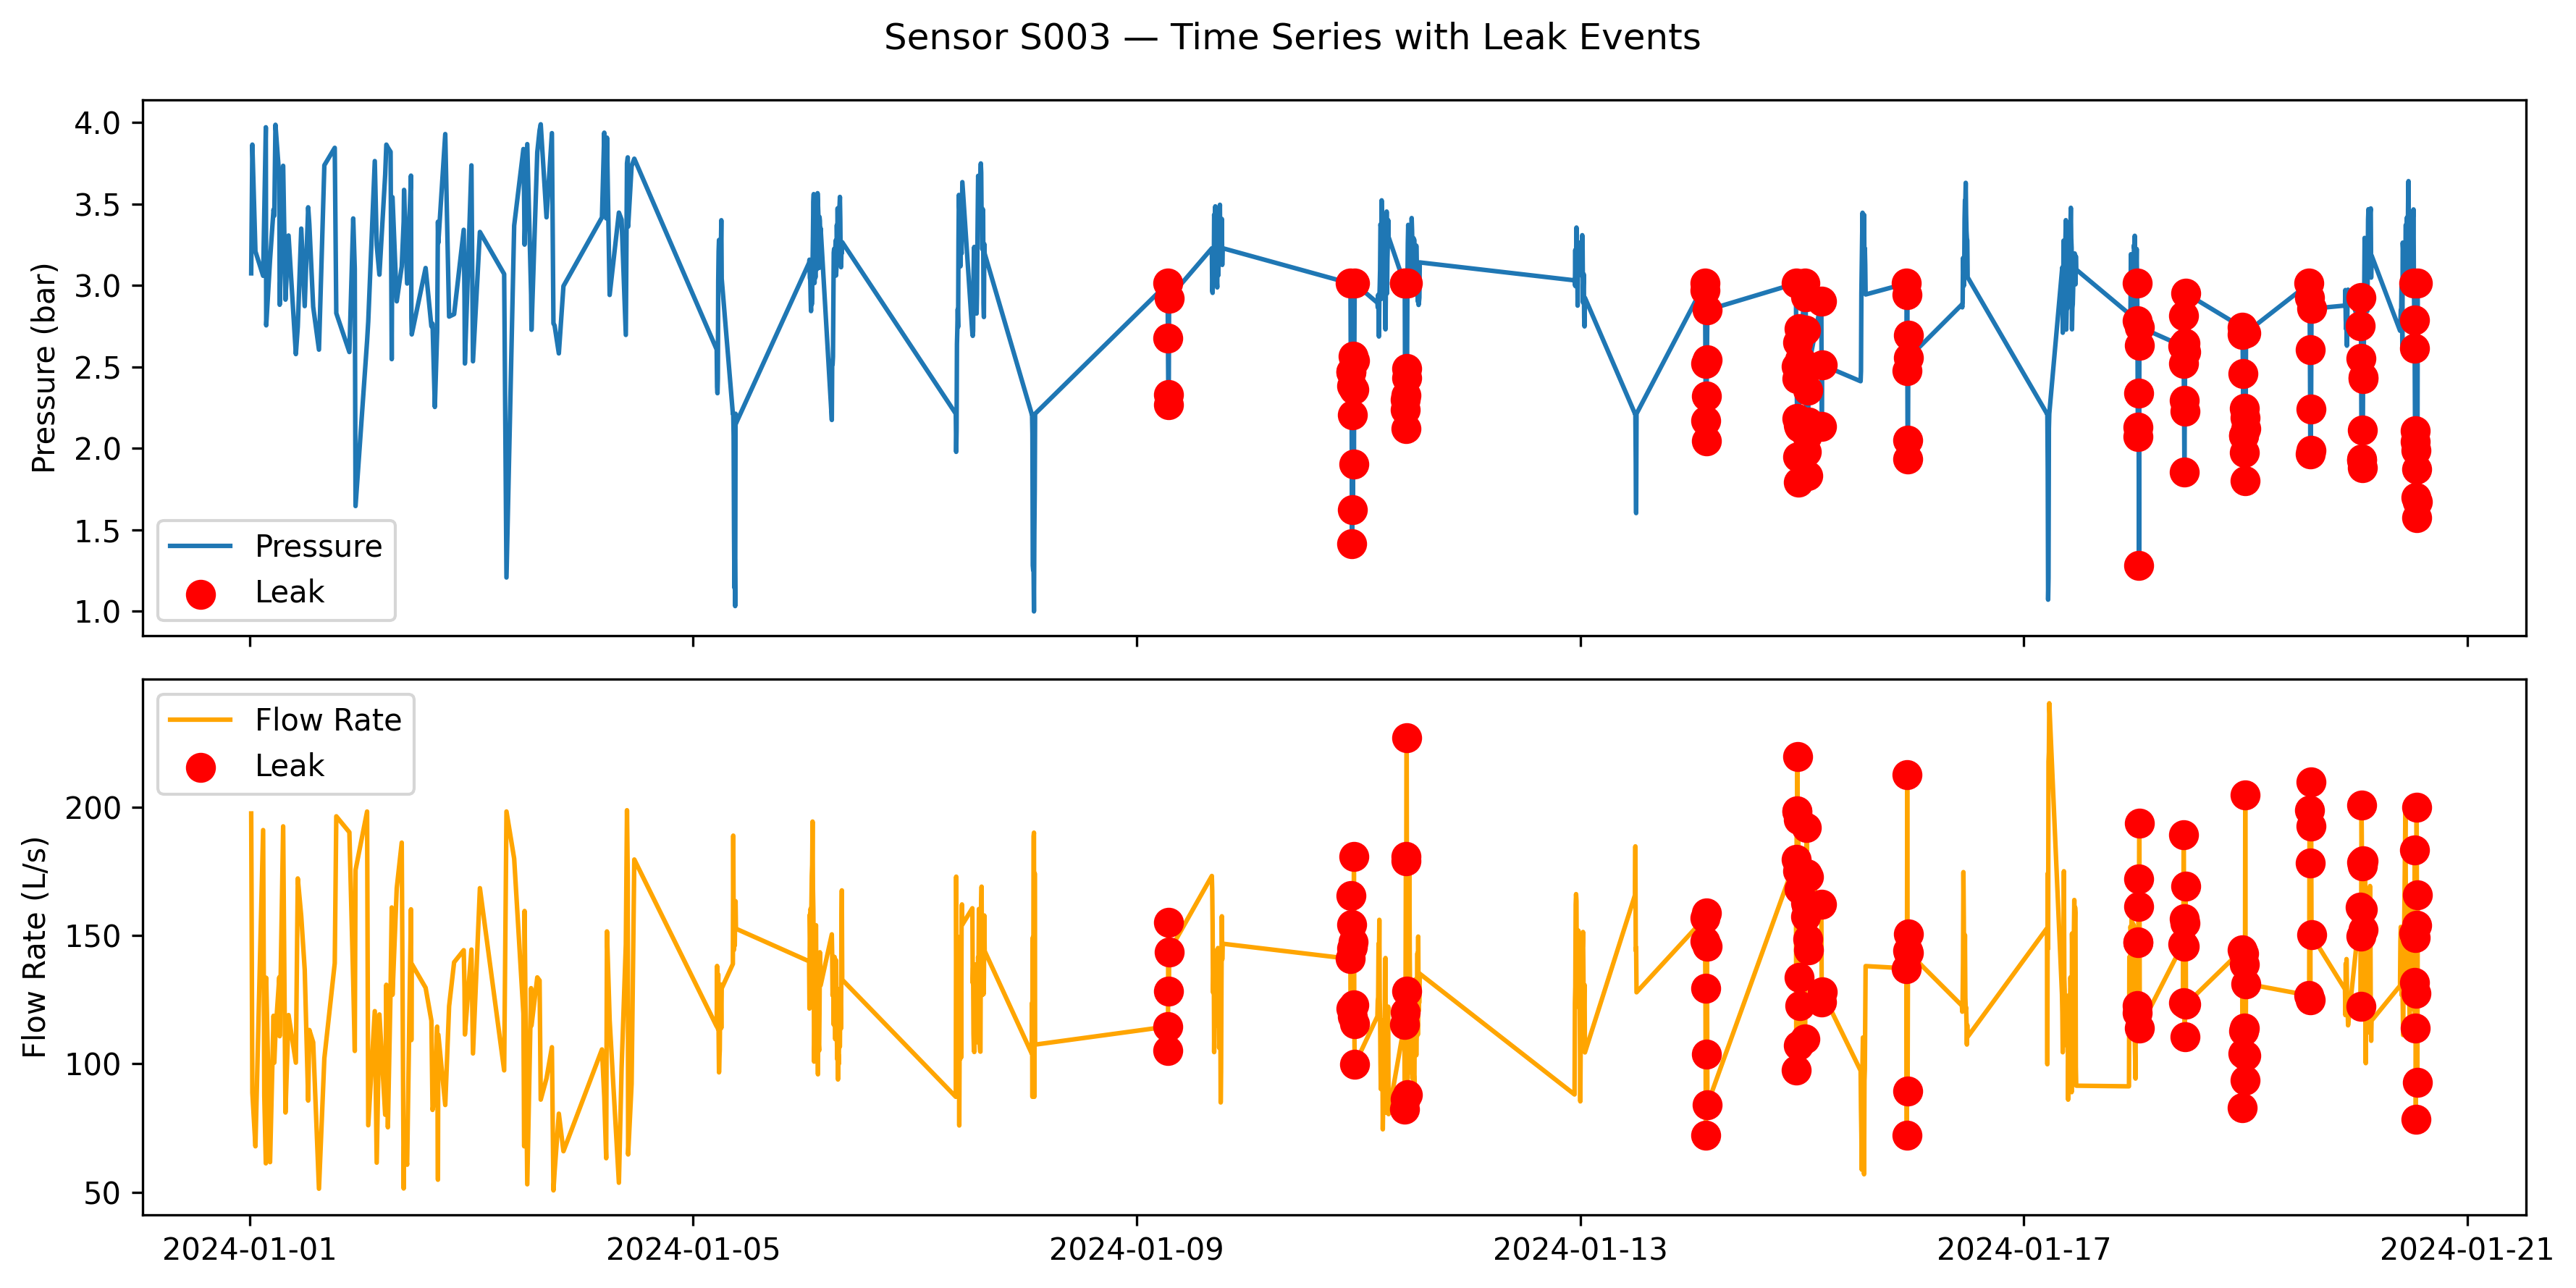
\includegraphics[width=\columnwidth]{images/fig3_timeseries_leak_sensor.png}
\caption{Exemple de série temporelle d'un capteur montrant les variations de
pression et de débit avec mise en évidence des événements de fuite.}
\label{fig:timeseries}
\end{figure}

La Figure~\ref{fig:timeseries} illustre l'évolution temporelle de la pression
et du débit pour un capteur représentatif. Les événements de fuite se manifestent
par des motifs temporels structurés, incluant des baisses de pression soutenues
et des fluctuations de débit corrélées. Ces observations montrent que la
détection des fuites ne peut pas être traitée comme un simple problème
d'anomalie ponctuelle, mais nécessite des modèles séquentiels capables de
capturer les dépendances temporelles.

\subsection{Analyse de corrélation des variables}

Pour quantifier les relations entre variables, nous calculons la matrice de
corrélation des principales caractéristiques.

\begin{figure}[h]
\centering
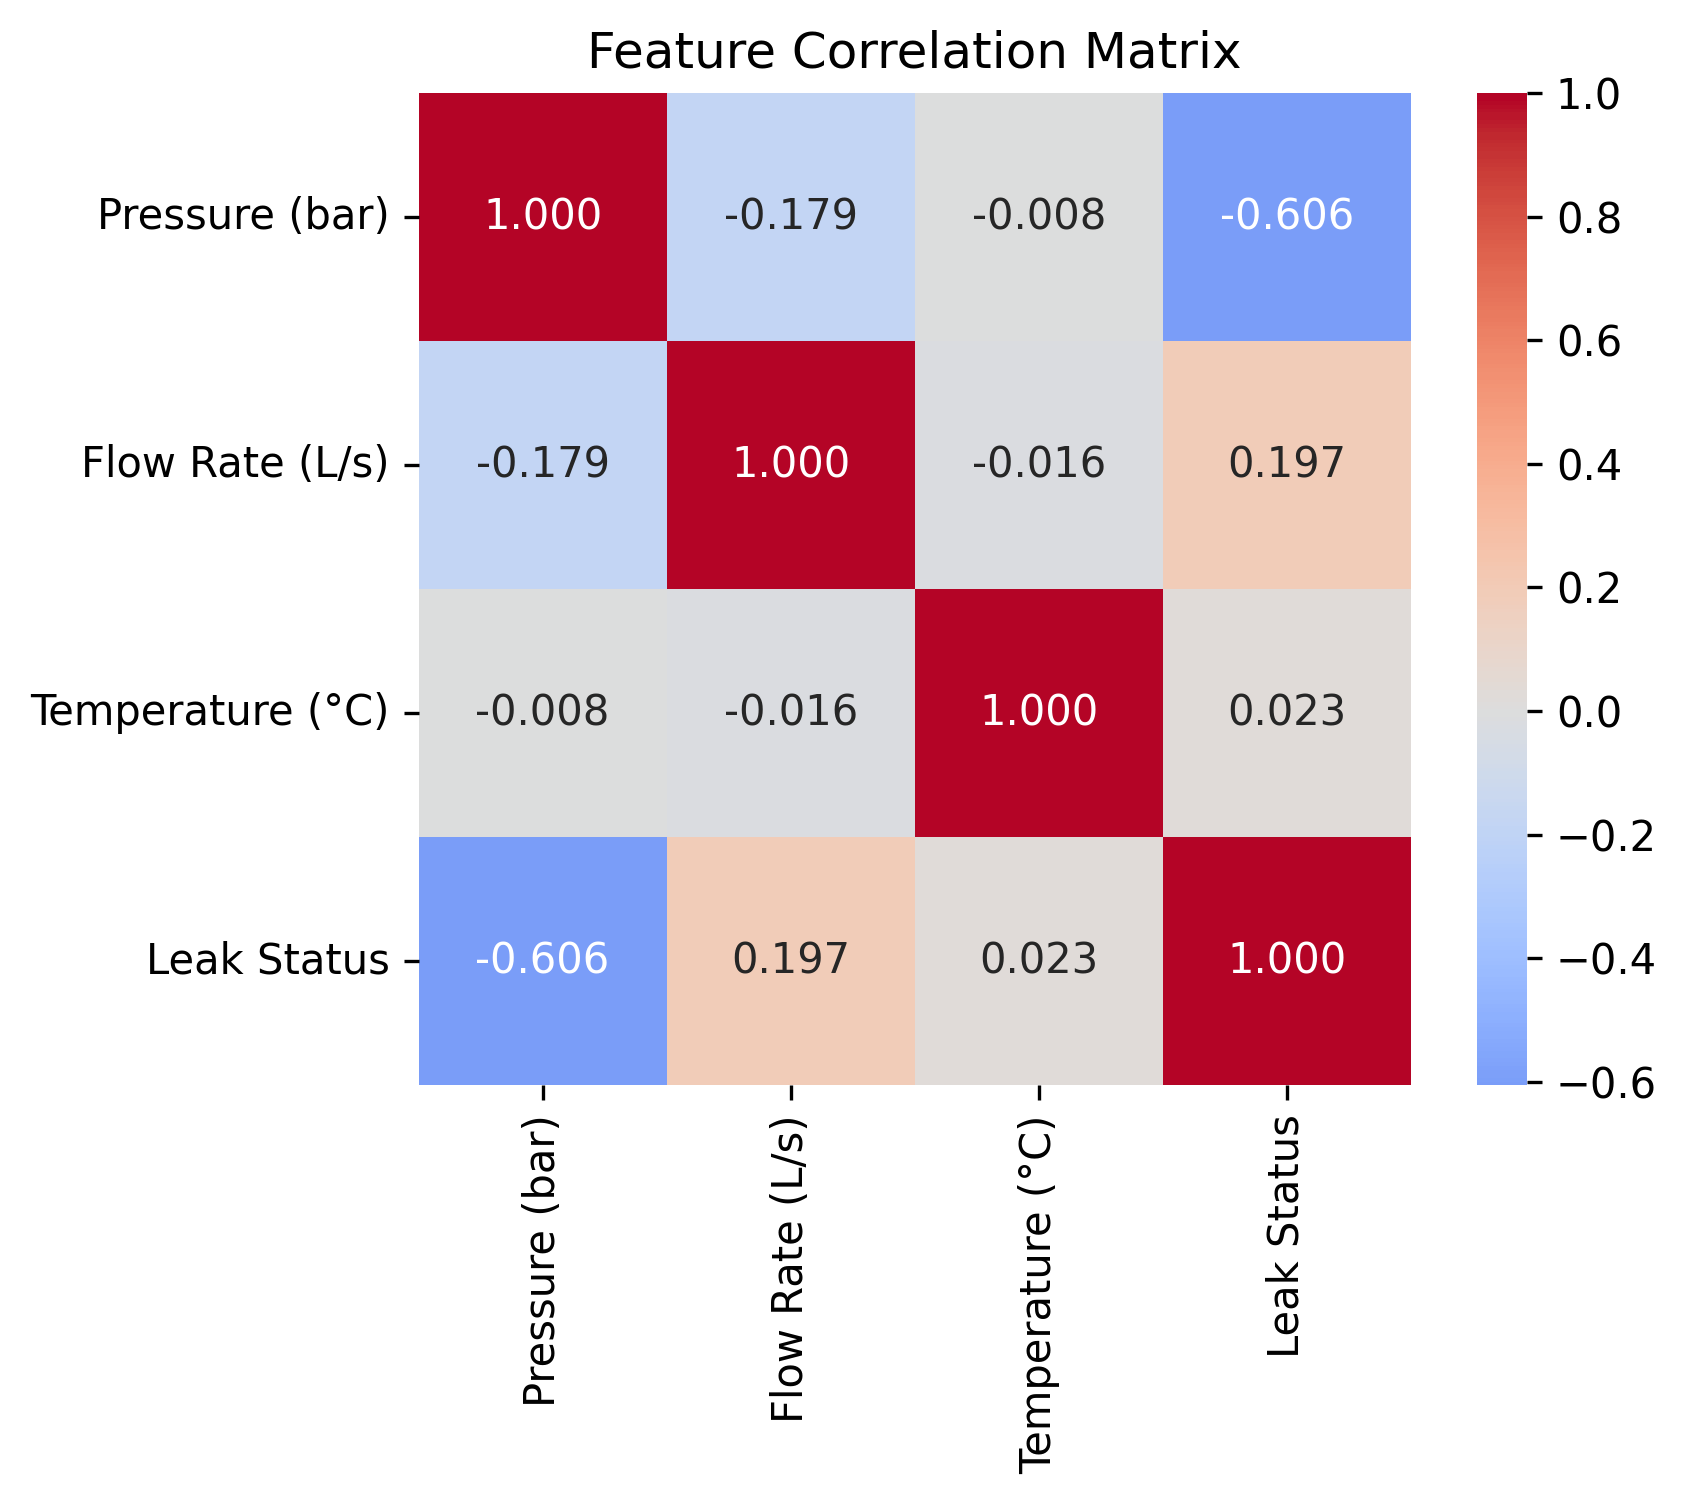
\includegraphics[width=0.9\columnwidth]{images/fig4_correlation_matrix.png}
\caption{Matrice de corrélation entre variables et état de fuite.}
\label{fig:correlation}
\end{figure}

Comme illustré à la Figure~\ref{fig:correlation}, la pression présente une
forte corrélation négative avec l'état de fuite ($-0.606$), confirmant son rôle
d'indicateur principal des événements de fuite. Le débit montre une corrélation
positive plus faible, tandis que la température présente une corrélation
négligeable, indiquant une influence directe limitée sur la détection.

Ces résultats suggèrent que, même si les variables individuelles fournissent des
signaux utiles, leurs relations sont intrinsèquement non linéaires et
interdépendantes, ce qui motive l'utilisation de modèles d'apprentissage avancés
capables de capturer ces interactions.

\subsection{Discussion}

L'analyse exploratoire met en évidence plusieurs caractéristiques clés du jeu
de données :

\begin{itemize}
    \item Les événements de fuite sont associés à une pression plus faible et à une variabilité du débit plus élevée.
    \item La structure temporelle est essentielle pour distinguer les motifs de fuite du comportement normal.
    \item Le jeu de données présente un déséquilibre de classes significatif, nécessitant des stratégies d'évaluation adaptées.
    \item Les relations linéaires seules sont insuffisantes pour capturer pleinement la dynamique des fuites.
\end{itemize}

Ces constats justifient l'utilisation d'architectures hybrides de deep learning
et d'approches de modélisation séquentielle. Ils motivent également la nécessité
d'une évaluation robuste et d'une comparaison avec des modèles alternatifs,
comme présenté dans les sections suivantes.